%Template pembuatan proposal skripsi.
\documentclass{jtetiproposalskripsi}

%-----------------------------------------------------------------
%Disini awal masukan untuk data proposal skripsi
%-----------------------------------------------------------------
\titleind{PERANCANGAN JARINGAN HOTSPOT SERVER BERBASIS MIKROTIK DI GEDUNG KULIAH UNIVERSITAS MUHAMMADIYAH JEMBER}

\fullname{NANANG CHAELANI}

\idnum{111065 1011}

\approvaldate{20 Desember 2014}

\degree{Sarjana Teknik Informatika}

\yearsubmit{2014}

\program{Teknik Informatika}

\headprogram{Sarjiya, S.T., M.T., Ph.D.}

\dept{Teknik Informatika}

\firstsupervisor{Sigit Basuki Wibowo, S.T., M.Eng.}
\firstnip{1976 0501 2002 12 1 002}

\secondsupervisor{Bimo Sunarfri Hantono, S.T., M.Eng.}
\secondnip{1977 0131 2002 12 1 003}


%-----------------------------------------------------------------
%Disini akhir masukan untuk data proposal skripsi
%-----------------------------------------------------------------

\begin{document}

\cover

\approvalpage

%-----------------------------------------------------------------
%Disini akhir masukan untuk muka skripsi
%-----------------------------------------------------------------

%-----------------------------------------------------------------
%Disini awal masukan Intisari
%-----------------------------------------------------------------
\begin{abstractind}
Komunikasi tanpa kabel/nirkabel (wireless) telah menjadi kebutuhan dasar atau gaya hidup baru masyarakat informasi. LAN nirkabel yang lebih dikenal dengan jaringan Wi-Fi menjadi teknologi alternatif dan relatif lebih mudah untuk diimplementasikan di lingkungan kerja. Instalasi perangkat jaringan Wi-Fi lebih fleksibel karena tidak membutuhkan penghubung kabel antar komputet. Access point  merupakan  perangkat  yang  biasa  digunakan  dalam  jaringan  wireless (Hotspot area) dimana user atau pengguna terhubung ke internet menggunakan media udara melalui perangkat access point. Selain itu, dengan jaringan berbasis wireless ini membuat masyarakat lebih mudah untuk mengakses internet dimanapun berada. Implementasi pemasangan jaringan ini terdiri dari pemasangan konektor RJ- 45 pada kabel UTP, melakukan konfigurasi repeater, konfigurasi Access Point, konfigurasi HotSpot Server MikroTik. Dengan adanya jaringan wireless berbasis HotSpot di Gedung Kuliah, akan mempermudah mahasiswa/i untuk mengakses internet dengan gratis. Selain itu, melakukan konfigurasi jaringan wireless tidak begitu sulit, asalkan mengikuti aturan pembuatan jaringan.

\bigskip
\textbf{Kata kunci} : Wireless, Tugas akhir, MikroTik, HotSpot, dan Access Point.
\end{abstractind}
%-----------------------------------------------------------------
%Disini akhir masukan Intisari
%-----------------------------------------------------------------

\tableofcontents
\addcontentsline{toc}{chapter}{DAFTAR ISI}
\selectlanguage{bahasa}\clearpage\pagenumbering{arabic}\setcounter{page}{1}

%-----------------------------------------------------------------
%Disini awal masukan untuk Bab
%-----------------------------------------------------------------
\chapter{LATAR BELAKANG}

\section{Latar Belakang Masalah}
Universitas  Muhammadiyah Jember  (UMJ)  merupakan  salah  satu  Perguruan Tinggi Swasta di jember yang terus berkembang menuju universitas terkemuka di Indonesia. Didirikan oleh Yayasan Muhammadiyah Jember, dengan tujuan membawa dampak yang positif dalam usaha pembangunan dan turut serta mencerdaskan bangsa melalui Tri Dharma Perguruan Tinggi. Dengan semangat pembaharuan, mengajak dan memberikan kesempatan kepada putra-putri terbaik di Indonesia untuk memacu prestasi dan meningkatkan kualitas generasi penerus bangsa Indonesia yang berilmu, beriman, dan bertaqwa melalui program-program pendidikan Strata Satu (S1), Diploma Tiga (D-III), dan Diploma Empat (D-IV) dalam berbagai disiplin ilmu pengetahuan. 



\section{Tujuan Penelitian}
Tujuan dari perancangan jaringan Hotspot ini adalah :

1.  Memudahkan mahasiswa untuk mengakses internet.

2. Mengetahui cara membangun jaringan Wireless menggunakan WDS (Wireless Distribution System).



\section{Manfaat Penelitian}
Adapun manfaat dari pembuatan sistem hotspot ini adalah untuk mengetahui sedikit tidaknya tentang konsep jaringan hotspot serta konfigurasinya dan sedikit mengetahui  kelebihan  dan  kekurangan  menggunakan  topologi  jaringan  WDS
(Wireless Distribution System).
 

%-------------------------------------------------------------------------------
\chapter{TINJAUAN PUSTAKA DAN DASAR TEORI}                

\section{Tinjauan Pustaka}
UMJ terdiri dari lulusan berkualitas dari berbagai perguruan tinggi ternama terbaik  dari  dalam  maupun luar negeri  yang mempunya  gelar akademi Doktor, Magister, dan Sarjana serta Spesialis dengan jenjang jabatan akademik: Lektor, Lektor Kepala dan Profesor.
Dengan luas kampus yang cukup besar, terdiri dari gedung-gedung kuliah yang dipenuhi oleh mahasiswa-mahasiswi, internet sudah menjadi salah satu kebutuhan pokok setiap hari untuk menggarap informasi. Maka dari itu disediakanlah fasilitas HotSpot bagi mahasiswa untuk mengakses internet.
Dewasa ini banyak system routing yang digunakan, dari yang gratis(free) sampai yang berbayar, dari mudah sampai yang susah dalam sistem konfigurasi- nya. Salah satunya yang akan kita bahas adalah MikroTik RouterOS, yaitu sistem operasi router yang sekarang ini banyak di gunakan oleh warnet-warnet, kantor- kantor ataupun instansi-instansi lain. MikroTik RouterOS merupakan router network  yang handal, dilengkapi dengan berbagai fitur dan tools, baik untuk jaringan kabel  maupun  jaringan tanpa kabel  (wireless). Salah satu fitur  yang disediakan oleh MikroTik yang akan di bahas adalah Hotspot Server

\section{Landasan Teori}
\subsection{Jaringan }
Sebuah   jaringan   terdiri   dari   2   atau   lebih   komputer   yang   saling berhubungan antara satu dengan yang lain, dan saling berbagi informasi.
Konsep jringan komputer lahir pada tahun 1940-an di Amerika, dari group riset Harvard University yang dipimpin oleh profesor H. Aiken. Pada mulanya proyek tersebut hanyalah ingin memanfaatkan sebuah perangkat komputer yang harus dipakai bersama. Untuk mengerjakan beberapa   proses tanpa banyak membuang waktu kosong maka dibuatlah proses beruntun (Batch Processing), sehingga  beberapa  program  bisa  di  jalankan  dalam  sebuah  komputer  dengan kaidah antrian. Ada beberapa jenis jaringan, yaitu :

1.  Local Area Network (LAN)

LAN adalah jaringan yang dibatasi oleh area yang relatif kecil, umumnya dibatasi oleh area lingkungan.
2.  Metropolitan Area Network (MAN)

MAN biasanya meliputi area yang lebih besar dari LAN, misalnya antar wilayah dalam satu propinsi yang menggabungkan jaringan LAN.
3.  Wide Area Network (WAN)

WAN  adalah  jaringan  yang  lingkupnya  biasanya  sudah  menggunakan sarana satelit ataupun kabel bawah laut.
(Andrian Tarigan,2009)



\subsection{WIFI}
Wi-Fi juga ditulis Wifi atau WiFi adalah sebuah teknologi terkenal yang memanfaatkan peralatan elektronik untuk bertukar data secara nirkabel (menggunakan gelombang radio) melalui sebuah jaringan komputer, termasuk koneksi  Internet  berkecepatan  tinggi.  Wi-Fi  Alliance  mendefinisikan  Wi-Fi sebagai "produk jaringan wilayah lokal nirkabel (WLAN) apapun yang didasarkan pada standar Institute of Electrical and Electronics Engineers (IEEE) 802.11". Meski  begitu,  karena  kebanyakan  WLAN  zaman  sekarang  didasarkan  pada standar tersebut, istilah  "Wi-Fi" dipakai dalam  bahasa  Inggris umum  sebagai sinonim "WLAN".

\subsection{WDS (Wireless Distribution System)}
Wireless Distribution System (WDS)  yang disebut juga sebagai Wireless Repeater merupakan sistem untuk mengembangkan jaringan nirkabel tanpa harus menggunakan kabel sebagai backbone untuk access point, melainkan memanfaatkan jalur nirkabel dari access point. Kekurangan repeater adalah bisa mengurangi performansi wireless LAN. Repeater harus menerima dan mengirim setiap frame pada kanal radio yang sama, mengakibatkan terjadinya peggandaan jumlah trafic pada jaringan. Hal ini terjadi jika digunakan banyak repeater. Untuk contoh topologi WDS dapat dilihat pada Gambar 2.1

\begin{figure}[ht!]
  \centering
    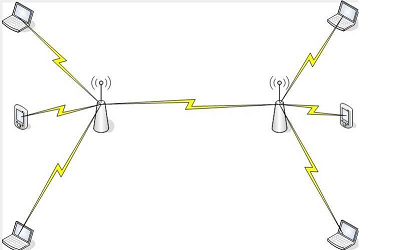
\includegraphics{gambar/1}
    \caption{Jaringan sensor nirkabel.}
    \label{1}
\end{figure}

\subsection{MikroTik RouterOS}
MikroTik RouterOS™ adalah sistem operasi dan perangkat lunak yang dapat  digunakan  untuk  menjadikan  komputer  manjadi  router  network  yang handal, mencakup berbagai fitur yang dibuat untuk ip network dan jaringan wireless, cocok digunakan oleh ISP dan provider hotspot.
MikroTik  adalah  perusahaan  kecil  berkantor  pusat  di  Latvia,  yang dibentuk oleh  John  Trully dan  Arnis  Riekstins.  Tahun  1996  John  dan  Arnis memulai dengan sistem Linux dan MS DOS yang dikombinasikan dengan teknologi Wireless LAN (W-LAN) Aeronet berkecepatan 2Mbps di Moldova. Barulah kemudian melayani lima pelanggannya di Latvia, karena ambisi mereka adalah membuat satu peranti lunak router yang handal dan disebarkan ke seluruh dunia.  Prinsip  dasar  MikroTik  bukan  membuat  Wireless  ISP  (WISP),  tapi membuat program router yang handal dan dapat dijalankan di seluruh dunia. Hingga kini, MikroTik telah melayani sekitar empat ratusan pelanggannya.Linux yang mereka gunakan pertama kali adalah Kernel 2.2 yang dikembangkan secara  bersama-sama dengan  bantuan  5  -  15  orang staf  R\&D Mikrotik yang sekarang menguasai dunia routing di negara-negara berkembang. Selain staf di lingkungan Mikrotik, menurut Arnis, mereka merekrut juga tenaga- tenaga lepas dan pihak ketiga yang dengan intensif mengembangkan Mikrotik secara maraton.( http://id.wikipedia.org/wiki/MikroTik)

\subsection{ HotSpot}
Hotspot (Wi-Fi) adalah salah satu bentuk pemanfaatan teknologi Wireless LAN  pada  lokasi-lokasi  publik  seperti  taman,  perpustakaan, restoran  ataupun bandara.  Pertama  kali  digagas  tahun  1993  oleh  Brett  Steward.  Hotspot  juga dikenal dengan istilah captive portal. Cactive Portal akan menagkap semuatrafik dari klien dan akan memeriksa apakah klien tersebut sudah terotentikasi atau belum untuk menggunakan sumber daya jaringan. Jika belum maka klien tersebut akan diperiksa untuk melakukan otentikasi terlebih dahulu.(Imam Cartealy,2013). 



Salah satu fitur terkenal di dalam mikrotik yang merupakan salah satu metode untuk memberikan akses/layanan internet di area public dengan melalui proses autentikasi seperti yang sudah disebutkan sebelumnya, media yang digunakan bisa menggunakan kabel ataupun wireless. Cara kerja dari hotspot server ini dalam bentuk sederhana, hotspot akan melakukan block semua akses user dan user akan diminta untuk melakukan login via web browser. Apabila username dan password yang diisikan oleh user cocok dengan database hotspot, maka layanan akses akan diberikan. Kami akan memberikan contoh konfigurasi bagaimana cara mengintegrasikan 2 hotspot server yang sudah ada di 2 router yang berbeda (router A dan router B) dengan sebuah database UserManager yang akan terpasang di salah satu router (router A). (http://mikrotik.co.id)

Topologinya bisa seperti yang ditunjukan pada Gambar 2.2 :

\begin{figure}[ht!]
  \centering
    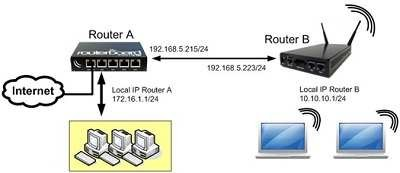
\includegraphics{gambar/2}
    \caption{Jaringan sensor nirkabel.}
    \label{2}
\end{figure}


%-------------------------------------------------------------------------------
\chapter{METODOLOGI}

\section{Alat dan Bahan}
Alat dan bahan yang digunakan dalam proses perancangan dan pembuatan HotSpot Server adalah sebagai berikut:


\vspace{-0.5cm}

\begin{enumerate}[1.]
\begin{singlespace}
\itemsep0em
\item Satu Unit PC/Laptop,
\item Router Board MikroTik RB450G / MikroTik RouterOS Level 4,
\item Access Point,
\item Kabel UTP Cat6 AMP,
\item Winbox,
\item Mozilla Firefox,
\end{singlespace}
\end{enumerate}

\section{Langkah Kerja}
Untuk mendapatkan data dan informasi yang baik dan tepat, maka penulis menggunakan teknik sebagai berikut:

\textbf{1. Studi Literatur}

Studi literatur adalah penelitian yang dilakukan untuk mendapatkan bahan rujukan berupa referensi yang bersifat teoristis dari buku-buku dan sumber bacaan lain yang dapat mendukung topik.

\textbf{2. Persiapan software}

Tahapan ini dilakukan persiapan softeware yang mendukung dalam perancangan sistem jaringan.

\textbf{3. Pengambilan data lapangan}

Data lapangan dibutuhkan sebagai data untuk perancangan jaringan Hotspot  dan dibutuhkan data mahasiswa untuk pembentukan  User Manager berupa NIM.

\textbf{4. Perancangan Jaringan}

Seluruh  informasi  dan  survey lapangan  akan  dirancang  membangun jaringan HotSpot

\textbf{5.Analisa Hasil Simulasi}

Tahapan ini merupakan tahapan analisa dari hasil uji coba serta melakukan perbaikan terhadap rancangan apabila ditemukan kekurangan atau kesalahan. 


\section{Jadwal Kegiatan}
Penelitian direncanakan akan dilaksanakan selama enam bulan. Rincian rencana jadwal penelitian dicantumkan dalam tabel berikut.

\begin{center}
Tabel 3.1. Jadwal Penelitian.
\end{center}
\vspace{-0.5cm}
\begin{figure}[ht!]
  \centering
    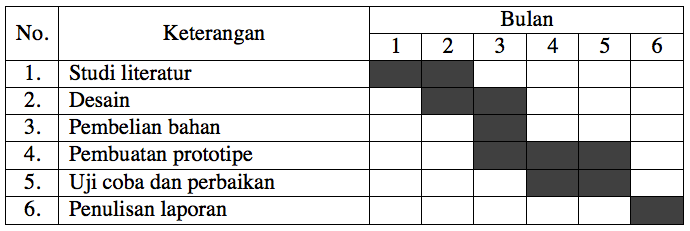
\includegraphics[width=13cm]{gambar/timeline}
\end{figure}

%-----------------------------------------------------------------
%Disini akhir masukan Bab
%-----------------------------------------------------------------

%-----------------------------------------------------------------
%Disini awal masukan untuk Daftar Pustaka
%-----------------------------------------------------------------
%%\nocite{Abel2010,Guerbas201350}
%%\bibliography{research-plan}
%%\bibliographystyle{plainnat}
\begin{thebibliography}{9}

\bibitem[satu(2014)]{satu01}

Cartealy, Imam. 2013. Tips \& Trik Mikrotik Router OS untuk SOHO ANDI Publisher: Yogyakarta


\bibitem[dua(2014)]{dua02}
Herlambang, Moch. Linto, Catur L, Azis. 2008. Panduan Lengkap Menguasai Router   Masa   Depan   Menggunakan   MikroTik   RouterOS™   .ANDI Publisher : Yogyakarta

\bibitem[tiga(2014)]{tiga03}
Tarigan, Andrian. 2009. Bikin Gateway Murah Pakai Mikrotik, Gramedia: Jakarta


\end{thebibliography}
\addcontentsline{toc}{chapter}{DAFTAR PUSTAKA}
%-----------------------------------------------------------------
%Disini akhir masukan Daftar Pustaka
%-----------------------------------------------------------------

\end{document}